\documentclass{standalone}
\usepackage[utf8]{inputenc}
\usepackage{pgfplots}
\usepgfplotslibrary{groupplots}
\usepgfplotslibrary{dateplot}
\pgfplotsset{compat=newest}
\usepackage{luatex85}
\begin{document}
% This file was created by tikzplotlib v0.9.0.
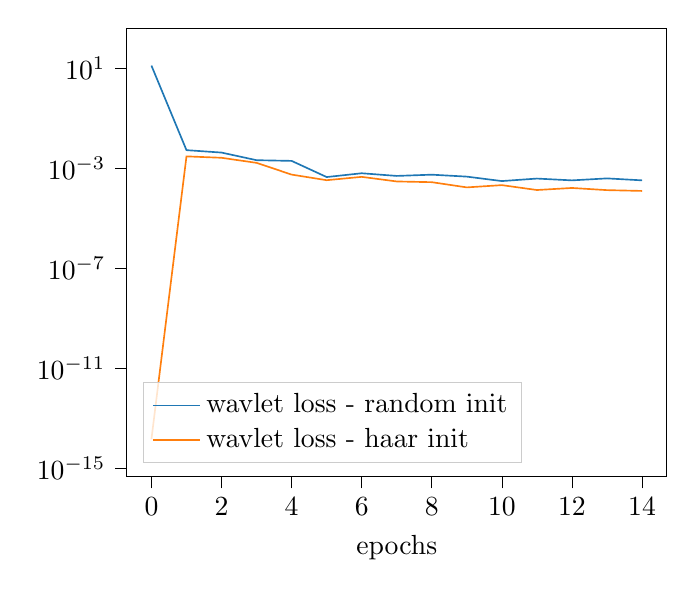
\begin{tikzpicture}

\definecolor{color0}{rgb}{0.12156862745098,0.466666666666667,0.705882352941177}
\definecolor{color1}{rgb}{1,0.498039215686275,0.0549019607843137}

\begin{axis}[
legend cell align={left},
legend style={fill opacity=0.8, draw opacity=1, text opacity=1, at={(0.03,0.03)}, anchor=south west, draw=white!80!black},
log basis y={10},
tick align=outside,
tick pos=left,
x grid style={white!69.0196078431373!black},
xmin=-0.7, xmax=14.7,
xtick style={color=black},
y grid style={white!69.0196078431373!black},
%ymin=0.000164165649299074, ymax=185.268038484793,
ymode=log,
ytick style={color=black},
%ytick={1e-05,0.0001,0.001,0.01,0.1,1,10,100,1000,10000},
%yticklabels={\(\displaystyle {10^{-5}}\),\(\displaystyle {10^{-4}}\),\(\displaystyle {10^{-3}}\),\(\displaystyle {10^{-2}}\),\(\displaystyle {10^{-1}}\),\(\displaystyle {10^{0}}\),\(\displaystyle {10^{1}}\),\(\displaystyle {10^{2}}\),\(\displaystyle {10^{3}}\),\(\displaystyle {10^{4}}\)},
xlabel={epochs}
]
\addplot [semithick, color0]
table {%
0 13.0555171966553
1 0.00536005571484566
2 0.00428549014031887
3 0.00212177890352905
4 0.00199133506976068
5 0.000448606122517958
6 0.000635871721897274
7 0.000497457338497043
8 0.000558379630092531
9 0.000466370023787022
10 0.000309311988530681
11 0.000389770895708352
12 0.00032995460787788
13 0.000395997922169045
14 0.000330628798110411
};
\addlegendentry{wavlet loss - random init}
\addplot [semithick, color1]
table {%
0 1.4210854715202e-14
1 0.00301781762391329
2 0.00264815427362919
3 0.0016594051849097
4 0.000562460510991514
5 0.000335427233949304
6 0.0004564261471387
7 0.000298629107419401
8 0.000279289844911546
9 0.000172741478309035
10 0.000212775776162744
11 0.000135634181788191
12 0.000163890887051821
13 0.000134164496557787
14 0.000124604644952342
};
\addlegendentry{wavlet loss - haar init}
\end{axis}

\end{tikzpicture}

\end{document}
